\graphicspath{ {./images/2_Data_import} }
\newpage

\section{Data import}\label{data_import}
\subsection{Raw data input}
In the \textsf{Upload your data} box, choose the type of raw data that you want to upload: LaCyTools data, Skyline data or SweetSuite data. 
Hovering over the blue info icon will show information about the formatting requirements. 
See the sections below for more details.

The uploaded data is converted into a clean data frame, with a column for each variable in the data.
The converted data is displayed in the top-right box \textsf{View the converted data} in the dashboard.

\begin{optionalbox}
	When applicable, specify keywords by which total and specific immunoglobulin samples can be recognized in the sample names.
	The specification is case sensitive.
	The table with converted data will be given an additional column called \textsf{group}, specifying whether a sample contains total or specific glycosylation data.
	Total and specific samples will be curated separately in later steps.
	\begin{center}
		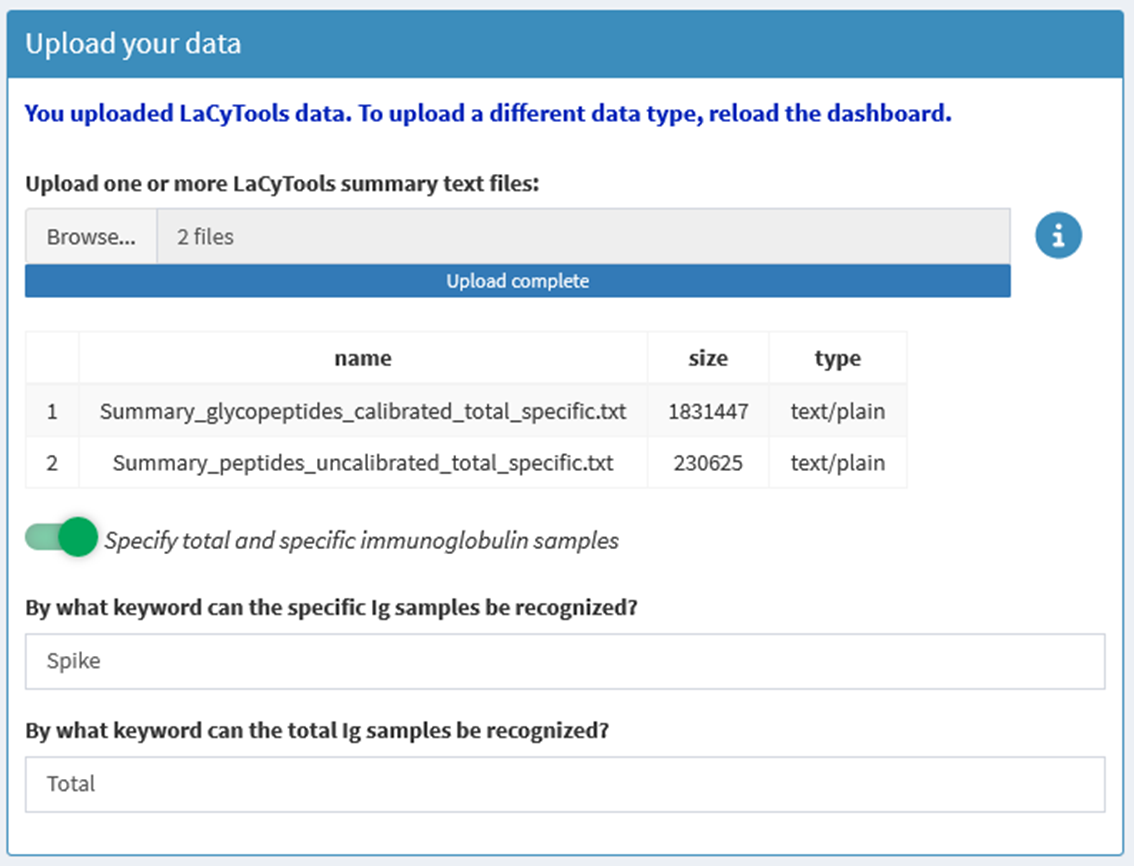
\includegraphics[width=0.62\linewidth]{import_lacytools.png}
	\end{center}
\end{optionalbox}

\subsubsection{Formatting of LaCyTools data}
You can upload one or more summary text files created by LaCyTools. 
The names and sizes of the uploaded files will be displayed in a table.
Each LaCyTools summary text file must contain at least the following outputs:

\begin{enumerate}[topsep=0pt, itemsep=0pt]
	\item Background subtracted absolute intensity
	\item Mass accuracy (ppm)
	\item Isotopic pattern quality (IPQ)
	\item Signal-to-noise ratio ($S/N$)
\end{enumerate}

These outputs should be present for each analyte, per charge state.

\subsubsection{Formatting of SweetSuite data}
SweetSuite creates an \texttt{.xlsx} file as output.
The \textsf{Data} sheet in this file contains several columns by default.
These \texttt{.xlsx} files can be uploaded directly into GlycoDash.

It is possible to upload multiple files at once.


\newpage
\subsubsection{Formatting of Skyline data (wide format)}
You can upload one \texttt{.csv} output file from Skyline.
The required formatting of the file depend on the way in which analytes are specified.
Analytes (glycopeptides) in the file must be specified in \emph{one of two ways}:

\begin{enumerate}[topsep=0pt, itemsep=0pt]
	% One column
	\item 
	\textbf{One column} where each entry contains both a peptide sequence and a glycan composition, e.g. \textsf{EEQYN[H3N4F1]STYR}.
	This column will likely be called either \textsf{Peptide Modified Sequence Full Names} or \textsf{Peptide Modified Sequence Three Letter Codes}.
	A sequence in this column may also contain methionine oxidation and cysteine carbamidomethyl (CAM) modifications.
	These modifications may be fully written out (\textsf{[Oxidation (M)], [Carbamidomethyl (C)]}), or they can be specified using a three letter abbreviation (\textsf{[Oxi], [CAM]}).
	\emph{Other modifications are currently not supported.}
	
	There must also be column containing protein names and a column specifying the charge states of the analytes.
	These columns will likely be called \textsf{Protein Name} and \textsf{Precursor Charge}, respectively.
	Additionally, the file should contains columns with \textsf{Total Area MS1}, \textsf{Isotope Dot Product} and \textsf{Average Mass Error PPM} \emph{for each sample name}.
	
	In the user interface, select the required columns and press the \menu{Process skyline data} button.
	
	Each unique combination of protein name and peptide sequence will be assigned a unique glycosylation site.
	The protein names will be converted to \textsf{PrA}, \textsf{PrB}, etc. in alphabetical order. 
	Peptide sequences will be abbreviated using the first three letters of the sequence. 
	When two or more peptides in a protein share the first three sequence letters, suffices (\textsf{\_a}, \textsf{\_b}, \textsf{\_c} etc.) are added to the sequence abbreviation.
	Finally, the protein and sequence abbreviations are pasted together with an underscore separating them, to form a string representing a unique glycosylation site.
	A downloadable table is generated where the protein names and peptide sequences can be linked to the assigned glycosylation sites. 
	
	\begin{center}
		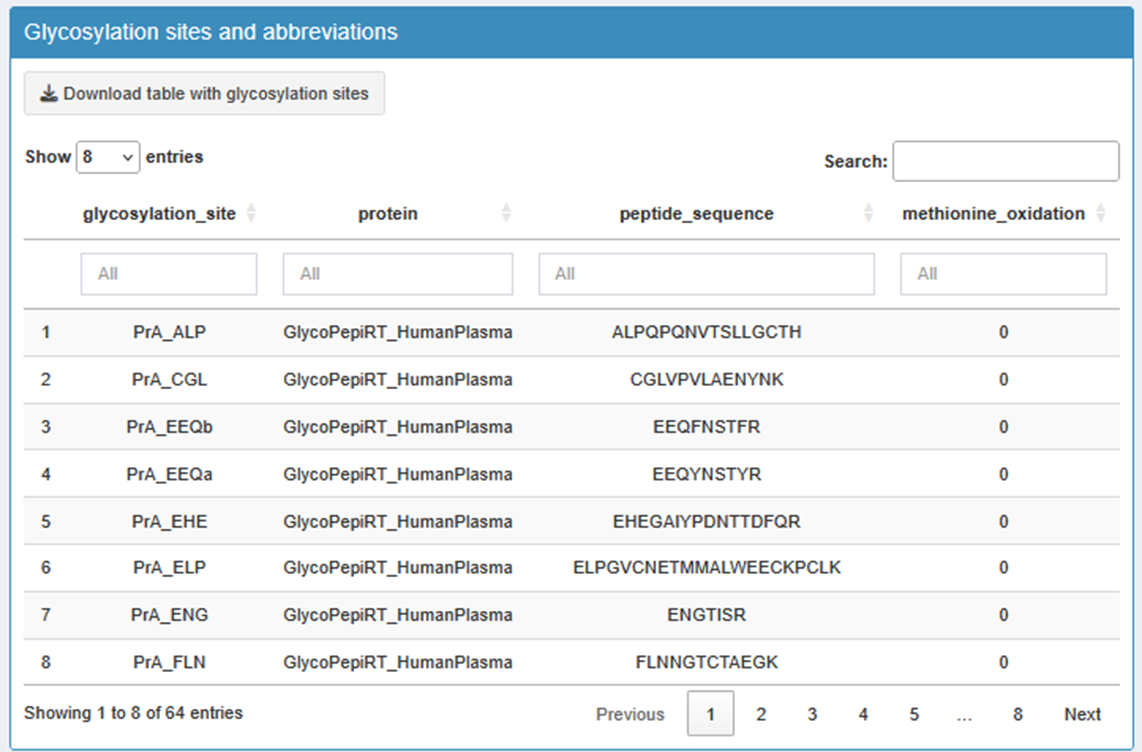
\includegraphics[scale=0.45]{skyline_peptides_table.png}
	\end{center}
	
	The column \textsf{methionine\_oxidation} lists the number of oxidized methionine residues in the corresponding peptide sequence.
	For each oxidized methionine, the \textsf{glycosylation\_site} entry is given an extra suffix \textsf{Ox}.
	
	% Two columns
	\item 
	\textbf{Two columns}, one with glycosylation sites and one containing glycan compositions.
	The glycosylation sites and glycans will be combined into a single analyte name (e.g., glycosylation site \textsf{PepI} and glycan \textsf{H3N4F1} will be combined into analyte \textsf{PepI1H3N4F1}).
	When analytes are specified this way, there must also be a column specifying the charge states of the analytes.
	This column will likely be called \textsf{Precursor Charge}.
	
	Additionally, the file should contain columns with \textsf{Total Area MS1}, \textsf{Isotope Dot Product} and \textsf{Average Mass Error PPM} \emph{for each sample name}.
	
	In the user interface, select the required columns and press \menu{Process skyline data} button.
		
\end{enumerate}


\begin{optionalbox}
	Skyline data may contain a column with notes for each analyte. 
	This column is likely called \textsf{Peptide Note}.
	After toggling the option \menu{Specify column with analyte notes} and selecting the corresponding column, an extra tab with notes for each analyte will be added to the output \texttt{.xlsx} file when exporting the processed data.
\end{optionalbox}

By default, analytes with isomeric glycan compositions are automatically detected and renamed when processing Skyline data.
For example, when \textsf{PepIH5N2} is present twice per sample (in each charge state), they are renamed to \textsf{PepIH5N2\_a} and \textsf{PepIH5N2\_b}. 
This renaming of isomers can be prevented by unchecking \menu{Automatically detect and rename glycan isomers}.



\subsubsection{Adding sample IDs}
Choose a method by which to add sample IDs:
\begin{itemize}[topsep=0pt, itemsep=0pt]
	\item 
	\textsf{Upload a plate design}  - This method requires each sample name to include a plate number and well position separated by an underscore. Examples of correctly formatted sample names are \textsf{MS\_\textbf{PL01\_B09}\_01\_2020.raw} and \textsf{IM1\_\textbf{PL02\_A11}\_03}.

	The plate design should be in \texttt{.xlsx} format, with different plates separated by an empty row.
	Each cell in the plate layout should contain a sample ID for the corresponding sample.
	If a plate well was not measured, the corresponding cell can be empty.
	Duplicate sample IDs are allowed to be present.
	An example of a plate design can be downloaded by clicking on the paperclip icon in the top-right corner of the \textsf{Add sample IDs} box.
	
	\begin{optionalbox}
		When applicable, you can upload separate plate layouts for total and specific immunoglobulin samples.
	\end{optionalbox}
	
	
	\item 
	\textsf{Upload a sample list} - Use this method when your sample names do not follow previously described format.
	The sample list should be a file in \texttt{.xlsx} format with the following two columns:
	\begin{enumerate}[topsep=0pt, itemsep=0pt]
		\item 
		\textsf{sample\_name} - This column should contain all the sample names that are present in the data (matching the names in the first column of the converted data).
		\item
		\textsf{sample\_id} - This column should contain the sample IDs corresponding to each sample name (e.g., \textsf{blank}, \textsf{pool}, \textsf{plasma}).
	\end{enumerate}
	An example of a sample list can be downloaded by clicking on the paperclip icon the top-right corner of the \textsf{Add sample IDs} box.
	
\end{itemize}

After uploading the required \texttt{.xlsx} file, a \textsf{sample\_id} column is automatically added to the converted data.


\newpage
\subsubsection{Adding sample types}
First choose a method to add sample types:
\begin{itemize}[topsep=0pt, itemsep=0pt]
	\item
	\textsf{Automatically} - Sample types are identified by finding common text patterns shared across sample IDs.
	For example, sample IDs \textsf{standard\_1} and \textsf{standard\_2} would both be assigned the sample type \textsf{standard}.
	\item 
	\textsf{Upload a list with sample types} - The uploaded list should a \texttt{.xlsx} file with two columns:
	\begin{itemize}[topsep=0pt, itemsep=0pt]
		\item 
		\textsf{sample\_id} - This column should contain each sample ID once (even if a sample ID appears multiple times in your data).
		\item 
		\textsf{sample\_type} - This column should specify the sample type corresponding to each sample ID.
		For instance, sample ID \textsf{PBS} could be assigned the sample type \textsf{blank}.
		Sample IDs \textsf{standard\_1} and \textsf{standard\_2} could be assigned the sample type \textsf{standard}.
		An example sample type file can be downloaded by clicking the paperclip button in the \textsf{Add sample types} box.
	\end{itemize}
\end{itemize}

Then, depending on your chosen method of adding sample types:
\begin{itemize}[topsep=0pt, itemsep=0pt]
	\item 
	\textsf{Automatically} - Click the \menu{Determine the sample types} button.
	A popup is shown with the detected sample types.
	To use these detected sample types, \menu{Accept these sample types}.
	If you want to use the other method instead, click \menu{Cancel}.
	\item 
	\textsf{Upload a list with sample types} - Upload your \texttt{.xlsx} file.
	The sample types will be added to the data automatically.
\end{itemize}


\subsubsection{Detection of glycosylation sites}
Glycopeptides in the data will automatically be assigned to glycosylation sites based on their names.
For example, two analytes \textsf{IgGI1H3N4F1} and \textsf{IgGI1H4N4F1} would both be assigned to the same glycosylation site \textsf{IgGI}.
Spectra curation and analyte curation will later be performed per glycosylation site.

\begin{optionalbox}
	Your data may contain heavy isotope labeled glycopeptides, such as SILuMAb IgG1 glycopeptides.
	These labeled glycopeptides will be assigned to glycosylation sites that are distinct from their natural counterparts.
\end{optionalbox}

Non-glycosylated peptides in your data are automatically detected. Two situations can occur:

\begin{itemize}[topsep=0pt, itemsep=0pt]
	\item 
	When there are glycopeptides whose glycosylation site corresponds to a non-glycosylated peptide, then this peptide can later be used for calculating site occupancies. 
	For example, if the analyte \textsf{IgGI1} is present in the the data, then this can be used to calculate the occupancy of glycosylation site \textsf{IgGI}.
	\item 
	When no corresponding glycopeptides exist in your data, then the non-glycosylated peptide is assumed to not be derived from a glycosylation site.
	These peptides can later be used for protein quantitation.
\end{itemize}
	

\subsubsection{Adding metadata (optional)}
You can upload a \texttt{.xlsx} file containing metadata such as age, sex and disease status.
This data will be merged with the glycosylation data.
This integration ensures that the final output data is ready for further data analysis in a program of your choice.
The metadata can later also be used to perform analyte curation per biological group.
The \texttt{.xlsx} file must contain one column with sample IDs, and additional columns with the metadata.





